\documentclass[oneside,a4paper,12pt, DIV=calc]{scrbook}
\usepackage{amsmath,amsfonts,amssymb,amsthm, tikz-cd, graphicx}
\usepackage[labelfont={bf},textfont=it]{caption}
\usepackage{subcaption}
\usepackage{booktabs}
\usepackage{algorithm}
\usepackage[noend]{algpseudocode}
\usepackage{parskip}
\usepackage[all]{nowidow}

\author{Daniel Collin}
\title{Brains and Bugs: Two Applications of Persistent Homology in the Life Sciences}
\newtheorem{theorem}{Theorem}
\newtheorem{lemma}[theorem]{Lemma}
\newtheorem{corollary}{Corollary}[theorem]
\theoremstyle{definition}
\newtheorem{definition}{Definition}
\newtheorem{example}{Example}

\begin{document}
\chapter{Summary of simplicial and homological analysis of Snudda network}
A \textbf{simplex} of dimension $n$ is defined by its \textbf{faces}, simplices in dimension $n-1$. The smallest dimension possible is $0$, which consists of vertices. A $1$-simplex is an edge and a $2$-simplex is a triangle with interior. The faces of a $2$-simplex are all its constituting edges that make up the triangle. A \textbf{simplicial complex} is a set of simplices such that if it contains a simplex $\sigma$ it also contains all the faces of $\sigma$.

A \textbf{$n$-cycle} in a simplicial complex is roughly a $n$-dimensional hole. A $0$-cycle is a connected component, a $1$-cycle is a hole in the traditional sense, a $2$-cycle is a cavity or void (the 3D equivalent of a hole) and so on for further dimensions. The \textbf{homology group} $H_{k}$ consists of all the $k$-cycles in a simplicial complex which are not \textbf{boundaries}. A boundary is a cycle which is part of a higher simplex, so for example if we have a $2$-simplex (a triangle with interior) the collection of its faces (the edges around the interior) is not in $H_{1}$ even though its a cycle since it is the boundary of the triangle.

The \textbf{$k$th Betti number} $\beta_{k}$ of a simplicial complex is the number of elements in $H_{k}$, i.e. the number of holes in a certain dimension.

By adding vertices and their corresponding higher order simplices according to the formula (starting from the lowest value, i.e. the highest degree vertex)

\[
  f(\sigma) = \begin{cases}
    -\deg(\sigma) & \text{if } \dim(\sigma) = 0 \\
    \max_{\tau \text{ is a face of } \sigma} \{ f(\tau) \} & \text{if } \dim(\sigma) > 0
  \end{cases}
\]

we can compute which holes in $H_{k}$ survive when adding new simplices. This is the lifetime of a $n$-dimensional hole and it is encoded with a persistence diagram as seen in Figure 1.3 with $x$-axis given by birth time and $y$-axis by death time of a hole.

To construct a simplicial complex on a directed graph such as the network generated by Snudda we use the following construction.
\begin{definition}
  A \textbf{directed clique} is a directed graph $G=(V,E)$ such that every vertex has at least an outgoing or incoming edge to every other vertex in the graph. \end{definition}


\begin{definition}
  Let G=\{V,E\} be a directed graph. The \textbf{directed flag complex} dFl(G) is defined to be the simplicial complex whose $k$-simplices are all directed cliques with vertices $v_{0},\dots,v_{k}$ such that $\forall i: v_{i} \in V$
  and $\forall i,j: i < j \implies (v_{i}, v_{j}) \in E$. The vertices $v_{0}, v_{k}$ are called the source and the sink of a $k$-simplex.
\end{definition}

\begin{figure}[ht]
  \centering
  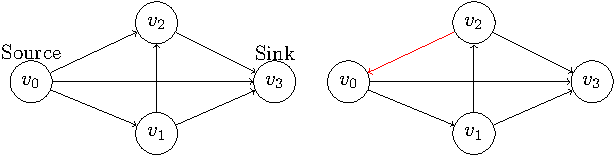
\includegraphics[]{./3simplex.pdf}
  \caption{\label{disimplex} Two directed cliques where the left clique does create a 3-simplex in the directed flag complex and the right clique does not.}
\end{figure}

In order to provide context, we compute three things for the network generated through Snudda together with 3 control models. In total we have four models: ST (Snudda, striatum), ER (Erdos-Renyi), WS (Watts-Strogatz), BA (Barasi-Albert). All of control models have their parameters set to be similar to ST in some way: for ER and WS we achieve approximately the same number of edges (and vertices) and for BA we achieve the same number of dimensions of simplices in the directed flag complex.

In Figure 1.2 we can see the total number of simplices in each dimension. ST has an abundance of simplices in each dimension compared to other models and more dimensions than ER and WS.

In Table 1.1 we see the Betti numbers for dimensions 1 and 2. ST has a much smaller number of $1$-dimensional holes (holes in the traditional sense) than any of the other networks. But in dimension two the number of holes grows rapidly while the control models do not change very much. It is likely this continues to higher dimensions.

Finally, in Figure 1.3 we see the lifetime of holes as we add vertices (and simplices containing those vertices when possible) in descending order of degree in $H_{0},H_{1}$ (connected components and normal holes). The distribution of holes is spread across the entire interval of possible degrees for ST, whereas for ER and WS this is concentrated around a specific region. (BA is not interesting in this aspect, since all vertices have pretty much the same degree)
\begin{figure}[ht]
  \centering
  \begin{subfigure}{.49 \linewidth}
    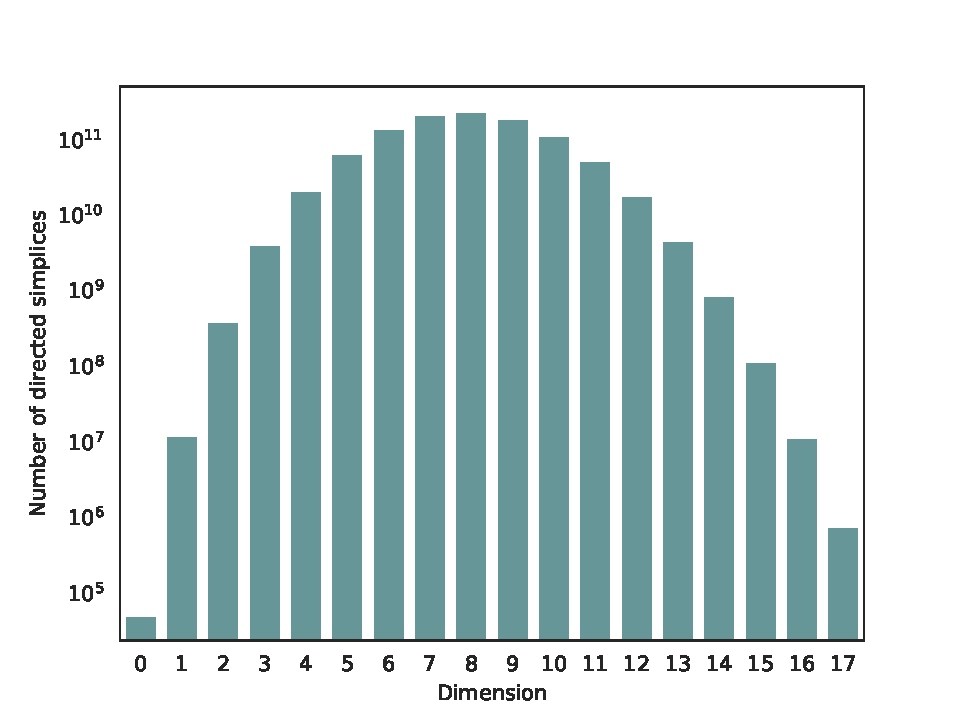
\includegraphics[scale=0.45]{./counts/real50k_count.pdf}
    \caption{ST}
  \end{subfigure}%
  \begin{subfigure}{.49 \linewidth}
    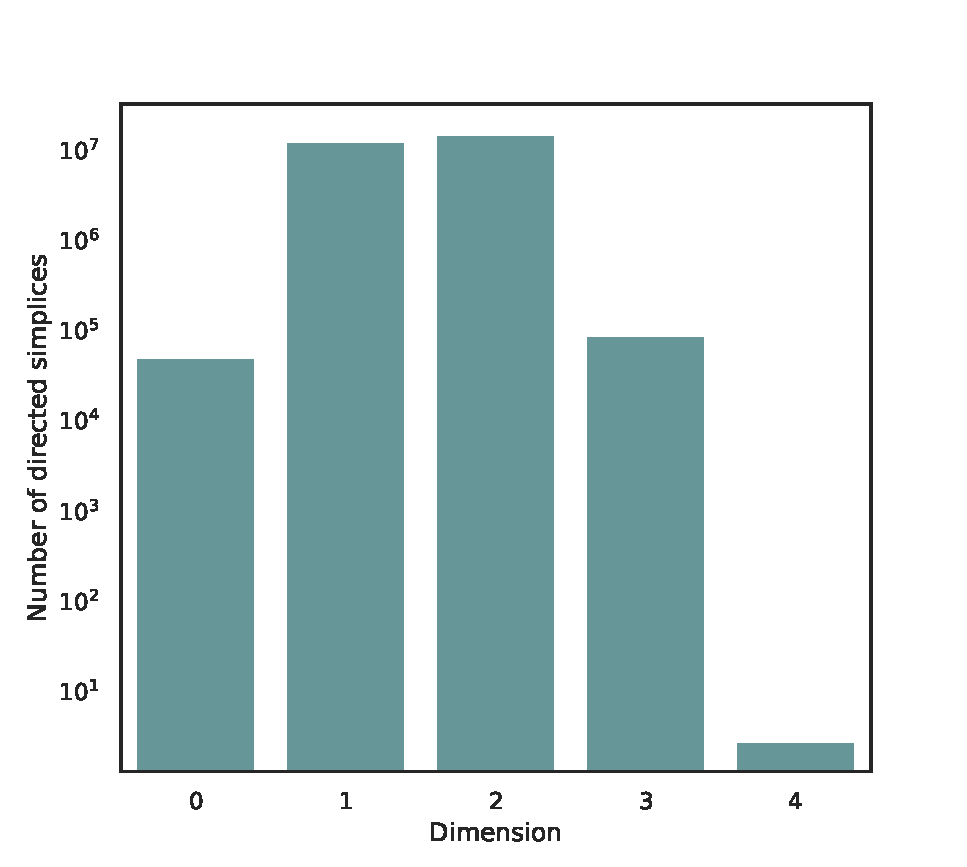
\includegraphics[scale=0.405]{./counts/random50k.pdf}
    \caption{ER}
  \end{subfigure}
  \begin{subfigure}{.45 \linewidth}
    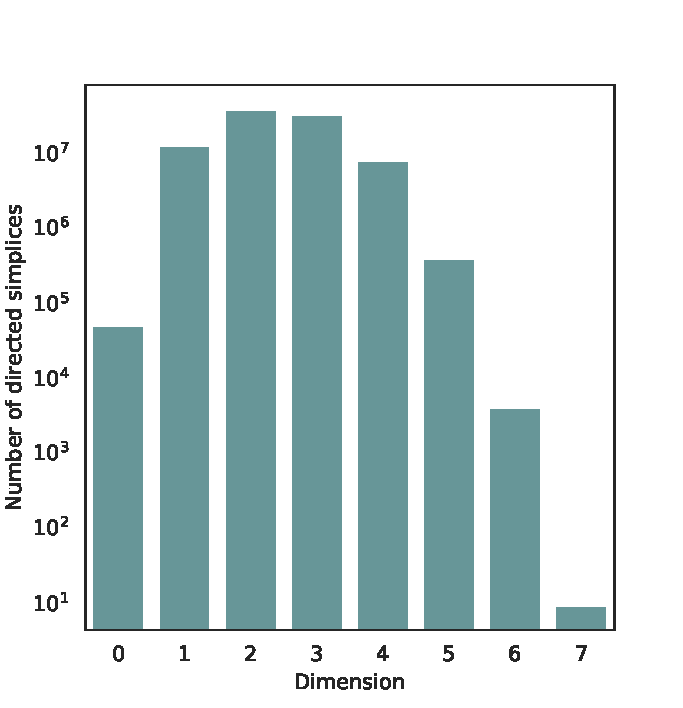
\includegraphics[scale=0.45]{./counts/random50k_ws_count.pdf}
    \caption{WS}
  \end{subfigure}
  \begin{subfigure}{.49 \linewidth}
    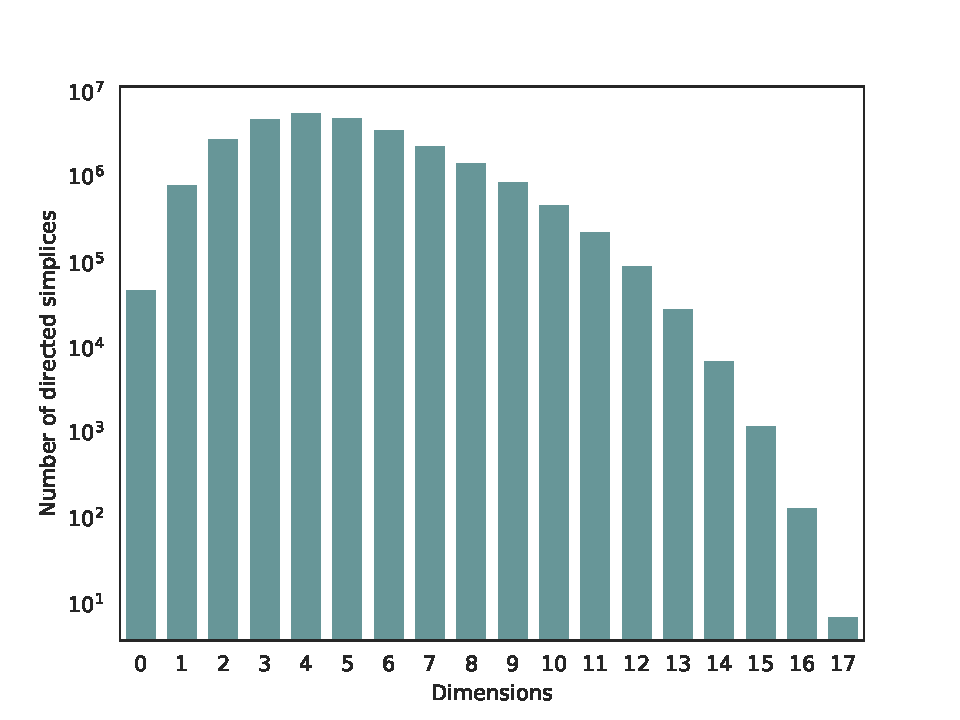
\includegraphics[scale=0.45]{./counts/random50k_ba_count.pdf}
    \caption{BA}
  \end{subfigure}
  \caption{\label{count50k}The total number of simplices in each dimension for the directed flag complex on ST, ER, WS and BA. For ER, WS and BA the counts are the result of the mean number of simplices in each dimension over 100 computations.}
\end{figure}

\begin{table}[ht]
\centering
\begin{tabular}{*4l}    \toprule
  Network & $\beta_{1} $  & $\beta_{2}$  & Computations \\ \toprule
  ST &   $5128 \pm 1219$ & $293013 \pm 79867$ & 1 \\
  ER &  $369770.18 \pm 687.69$ & $3470380.91 \pm 2774.23$ & 100 \\
  WS & $334754.93 \pm 625.38$ & $3756595.22 \pm 3709.97$ & 100 \\
  BA &  $11982.51 \pm 956.18$ & $12946.77  \pm 1734.00$ & 100
  \\
  \bottomrule
\end{tabular}
\caption{\label{bettis} Table over the first and second Betti numbers for the graphs ST, ER, WS and BA.}
\end{table}

\begin{figure}[ht]
  \centering

  \begin{subfigure}{.49 \linewidth}
    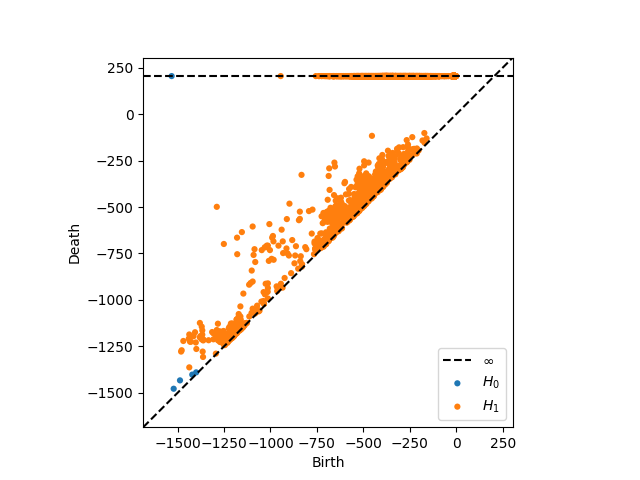
\includegraphics[scale=0.49]{./graph_phs/ST.png}
    \caption{ST}
  \end{subfigure}%
  \begin{subfigure}{.49 \linewidth}
    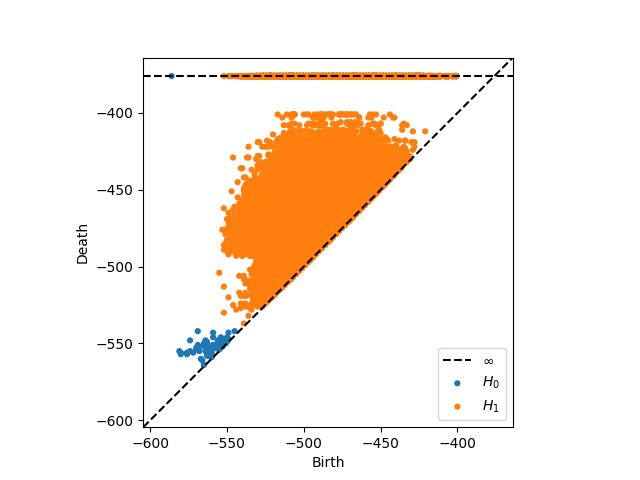
\includegraphics[scale=0.49]{./graph_phs/ER.png}
    \caption{ER}
  \end{subfigure}
  \begin{subfigure}{.49 \linewidth}
    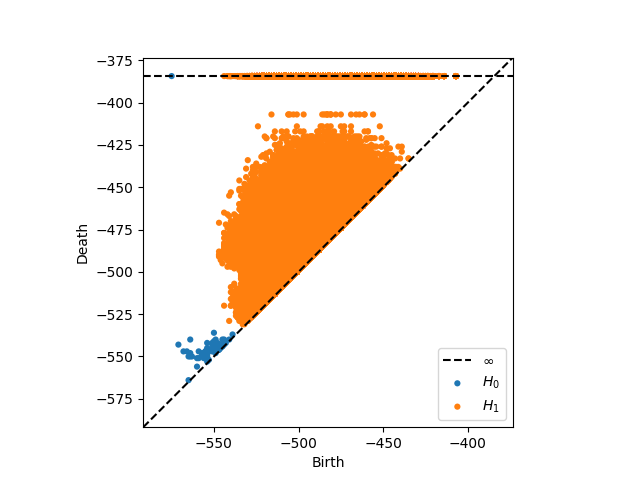
\includegraphics[scale=0.49]{./graph_phs/WG.png}
    \caption{WS}
  \end{subfigure}
  \begin{subfigure}{.49 \linewidth}
    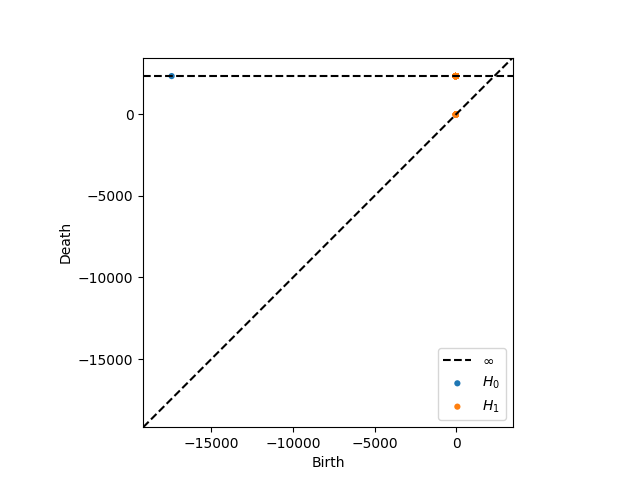
\includegraphics[scale=0.49]{./graph_phs/BA.png}
    \caption{BA}
  \end{subfigure}
  \caption{\label{graphph} Persistence diagrams over $H_{0}$ and $H_{1}$ for ST,ER,WS and BA given by inclusion of vertices and their resulting higher order simplices in the negative order of their degrees.}
\end{figure}
\end{document}
